The experiments used the pHopt enzyme optimal-pH dataset released with EpHod \citep{gado2023phopt,gado2025machine}. The source file, \texttt{data/raw/pHopt\_data.csv}, was downloaded from Zenodo record \texttt{10.5281/zenodo.14252615} (version 1; accessed 2026-10-22) under the CC BY 4.0 license. The file contains protein accessions, organism names, EC numbers, experimentally measured optimal-pH values, dataset-provided split labels, and amino-acid sequences. Its published MD5 checksum is \texttt{d5d0887710e70f2aa5153c15178a6d08}; the local SHA-256 checksum is \texttt{6C2CE7F68E28E4130904A96FC071DBF7FE78E090BD1E408408038F01FA75A3E9}.

The raw dataset contained 9855 records. No records were removed during the initial cleaning pass: there were no missing sequences, no missing optimal-pH values, no invalid sequence symbols, and no pH values outside the configured range from 0 to 14. The cleaned dataset therefore also contained 9855 records. Sequence length ranged from 33 to 1021 amino acids, with a median length of 396 and a mean length of 427.49. Experimental optimal pH ranged from 1.0 to 12.0, with a median of 7.5 and a mean of 7.2214.

Metadata coverage was sufficient for organism-held-out and EC-based subgroup analyses. The dataset contained 2346 unique organism labels and 3050 unique EC-number labels. The most frequent organism label was \textit{Homo sapiens} with 759 records, followed by \textit{Arabidopsis thaliana} with 368 records and \textit{Escherichia coli} with 318 records. The taxonomy column configured for the project was not present, so taxonomy-level splits beyond organism labels were not run.

Data validation identified 81 exact duplicate sequences and 41 exact duplicate sequences with conflicting pH labels. These records were retained for the current experiments but explicitly controlled in the exact-duplicate-safe and cluster-safe split definitions. Fifty sequences contained ambiguous residues, and these were retained with explicit reporting.

\begin{figure}[htbp]
    \centering
    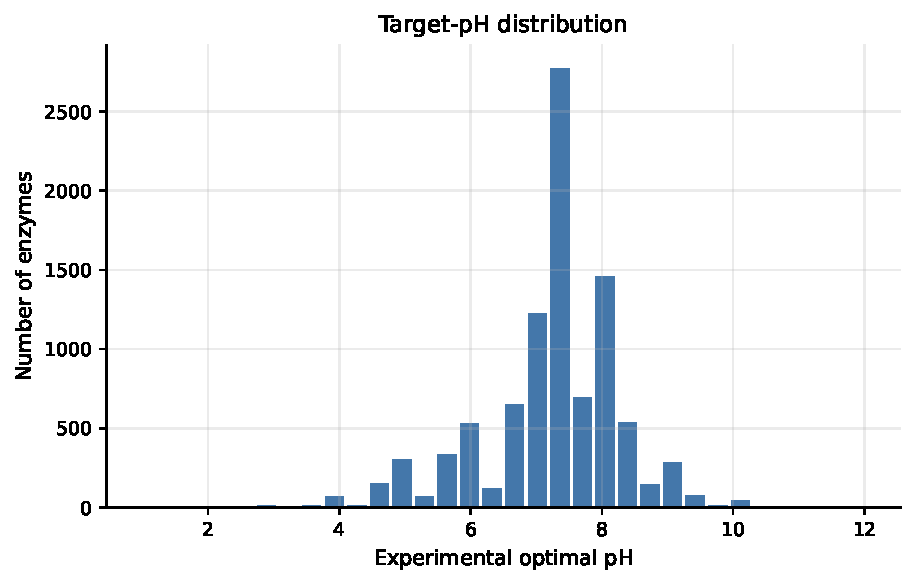
\includegraphics[width=0.78\textwidth]{figures/target_ph_distribution.pdf}
    \caption{Distribution of experimentally measured enzyme optimal-pH values in the cleaned dataset.}
    \label{fig:target-ph-distribution}
\end{figure}

\begin{figure}[htbp]
    \centering
    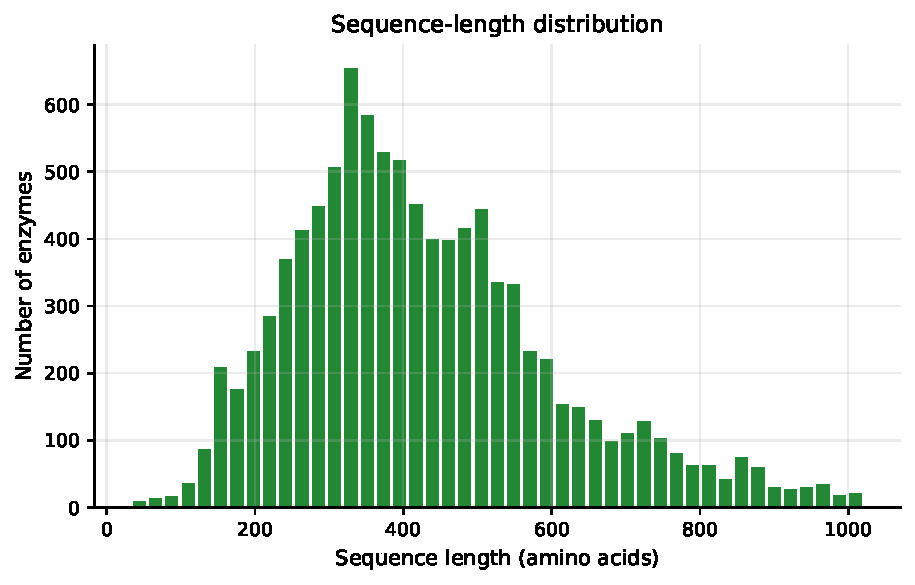
\includegraphics[width=0.78\textwidth]{figures/sequence_length_distribution.pdf}
    \caption{Distribution of amino-acid sequence lengths in the cleaned dataset.}
    \label{fig:sequence-length-distribution}
\end{figure}

\begin{figure}[htbp]
    \centering
    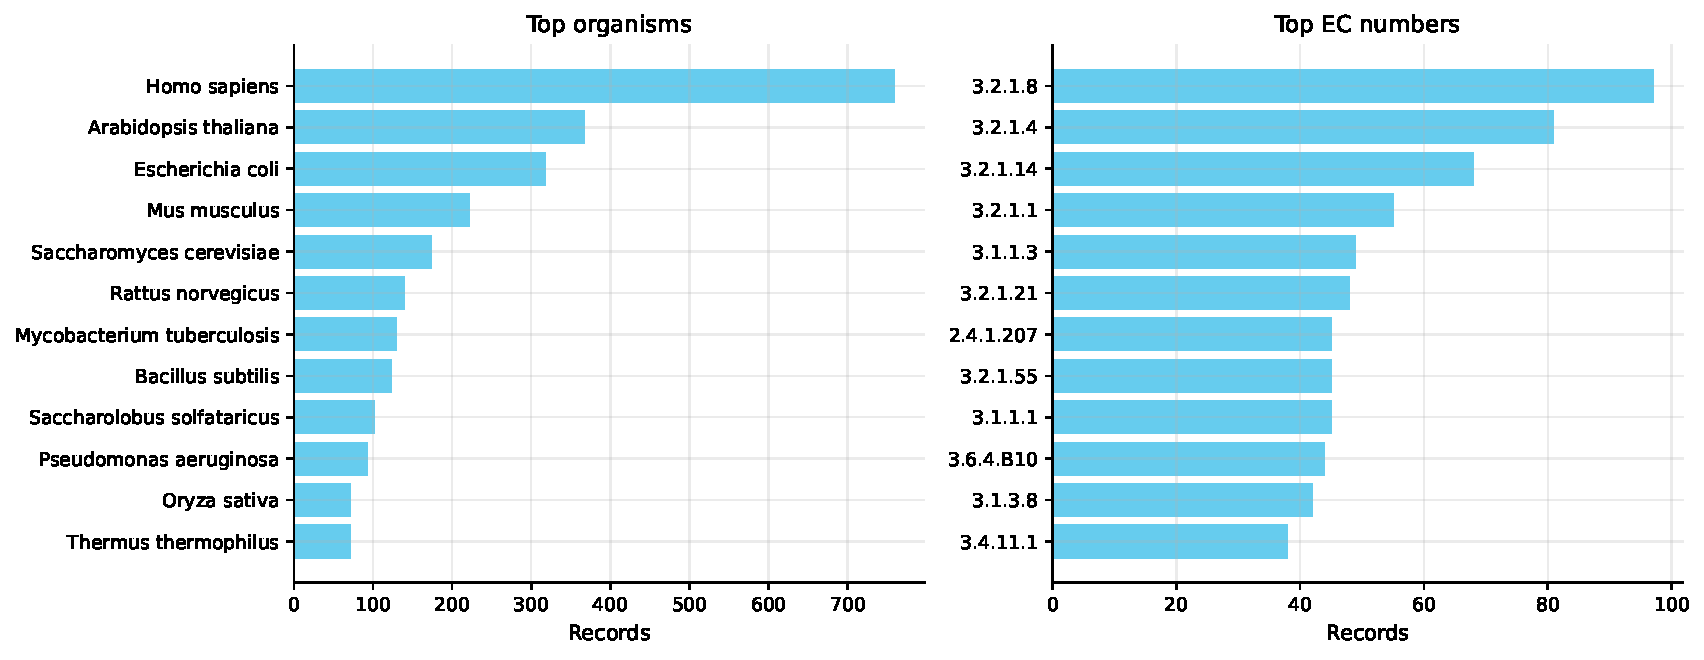
\includegraphics[width=\textwidth]{figures/dataset_composition.pdf}
    \caption{Most frequent organism and EC-number labels in the cleaned dataset.}
    \label{fig:dataset-composition}
\end{figure}
